
\documentclass[10pt,a4paper,twocolumn,twoside]{article}
\usepackage[utf8]{inputenc}
\usepackage[catalan]{babel}
\usepackage{multicol}
\usepackage{graphicx}
\usepackage{fancyhdr}
\usepackage{times}
\usepackage{titlesec}
\usepackage{multirow}
\usepackage{lettrine}
\usepackage[top=2cm, bottom=1.5cm, left=2cm, right=2cm]{geometry}
\usepackage[figurename=Fig.,tablename=TAULA]{caption}
\captionsetup[table]{textfont=sc}
% \usepackage{urlbst}
\usepackage{hyperref}


\author{\LARGE\sffamily Pol Colomer Campoy}
\title{\Huge{\sffamily Desenvolupament d'una Plataforma per a l'Anàlisi i Generació de Partitures Musicals a partir d'Àudio Multitrack}}


\newcommand\blfootnote[1]{%
  \begingroup
  \renewcommand\thefootnote{}\footnote{#1}%
  \addtocounter{footnote}{-1}%
  \endgroup
}

%
%\large\bfseries\sffamily
\titleformat{\section}
{\large\sffamily\scshape\bfseries}
{\textbf{\thesection}}{1em}{}

\begin{document}

\fancyhead[LO]{\scriptsize Pol Colomer Campoy: Desenvolupament d'una Plataforma per a l'Anàlisi i Generació de Partitures Musicals a partir d'Àudio Multitrack}
\fancyhead[RO]{\thepage}
\fancyhead[LE]{\thepage}
\fancyhead[RE]{\scriptsize EE/UAB TFG INFORMÀTICA: Desenvolupament d'una Plataforma per a l'Anàlisi i Generació de Partitures Musicals a partir d'Àudio Multitrack}

\fancyfoot[CO,CE]{}

\fancypagestyle{primerapagina}
{
   \fancyhf{}
   \fancyhead[L]{\scriptsize TFG EN ENGINYERIA INFORMÀTICA, ESCOLA D'ENGINYERIA (EE), UNIVERSITAT AUTÒNOMA DE BARCELONA (UAB)}
   \fancyfoot[C]{\scriptsize Juny de 2024, Escola d'Enginyeria (UAB)}
}

%\lhead{\thepage}
%\chead{}
%\rhead{\tiny EE/UAB TFG INFORMÀTICA: TÍTOL (ABREUJAT SI ÉS MOLT LLARG)}
%\lhead{ EE/UAB \thepage}
%\lfoot{}
%\cfoot{\tiny{Mes 2024, Escola d'Enginyeria (UAB)}}
%\rfoot{}
\renewcommand{\headrulewidth}{0pt}
\renewcommand{\footrulewidth}{0pt}
\pagestyle{fancy}

%\thispagestyle{myheadings}
\twocolumn[\begin{@twocolumnfalse}

%\vspace*{-1cm}{\scriptsize TFG EN ENGINYERIA INFORMÀTICA, ESCOLA D'ENGINYERIA (EE), UNIVERSITAT AUTÒNOMA DE BARCELONA (UAB)}

\maketitle

\thispagestyle{primerapagina}
%\twocolumn[\begin{@twocolumnfalse}
%\maketitle
%\begin{abstract}
\begin{center}
\parbox{0.915\textwidth}
{\sffamily
\textbf{Resum--}

Aquest treball es centra en la separació de pistes d'un fitxer d'àudio multitrack, on cada pista representa un instrument. S'utilitzen tècniques d'Anàlisi de Components Independents (ICA) i una arquitectura U-Net per a aquest propòsit. L'objectiu és generar automàticament la partitura de cada pista separada. Es realitza un anàlisi dels resultats i del rendiment dels algoritmes utilitzats, amb l'objectiu de concloure sobre les seves aplicacions en aquest sector.

\\
\\
\textbf{Paraules clau-- } Anàlisi de Components Independents (ICA), CNN, Espectrograma, Ground Truth, ML, Multitrack, separació d'àudio, U-Net.\\
\\
%\end{abstract}
%\bigskip
%\begin{abstract}
\bigskip
\\
\textbf{Abstract--} 
This work focuses on separating tracks from a multitrack audio file, where each track represents an instrument. Independent Component Analysis (ICA) and a U-Net architecture are employed for this purpose. The goal is to automatically generate the sheet music for each separated track. An analysis of the results and the performance of the algorithms used is conducted to draw conclusions on their applications in this field.

\\
\\
\textbf{Keywords-- } Audio decomposition, CNN, Ground Truth, ICA, ML, Multitrack, Spectrogram, U-Net.\\
}

\bigskip

{\vrule depth 0pt height 0.5pt width 4cm\hspace{7.5pt}%
\raisebox{-3.5pt}{\fontfamily{pzd}\fontencoding{U}\fontseries{m}\fontshape{n}\fontsize{11}{12}\selectfont\char70}%
\hspace{7.5pt}\vrule depth 0pt height 0.5pt width 4cm\relax}

\end{center}

\bigskip
%\end{abstract}
\end{@twocolumnfalse}]

\blfootnote{$\bullet$ E-mail de contacte: Pol.ColomerC@autonoma.cat}
\blfootnote{$\bullet$ Menció realitzada: Computació}
\blfootnote{$\bullet$ Treball tutoritzat per: Felipe Lumbreras (departament - CVC)}
\blfootnote{$\bullet$ Curs 2023/2024}


\section{Introducció - Context del treball}
\label{sec:intro}

\lettrine[lines=3]{E}{n} els darrers anys, el camp de l'enginyeria informàtica ha experimentat un notable avanç en el tractament del senyal d'àudio i en l'anàlisi musical automatitzada. El present projecte d'enginyeria informàtica, que implica la separació d'instruments, la generació de partitures i la creació de tutorials visuals, s'ubica en la intersecció de diverses àrees de recerca i desenvolupament. La meva principal motivació és adquirir pràctica i comprensió en l'àmbit de l'àudio, un tema menys explorat durant la meva carrera. Així, pretenc enriquir la meva experiència acadèmica en aquest camp. Aquest treball es centra en l'ús de l'Anàlisi de Components Independents (ICA) i l'arquitectura U-Net per a la separació de pistes en àudio multitrack, amb l'objectiu final de generar partitures musicals automàticament.



\section{Objectius}
\label{sec:objectius}

L'objectiu principal d'aquest projecte és aconseguir la separació de pistes d'àudio d'un arxiu multitrack i obtenir les notes musicals de cada pista per a la posterior generació de la seva partitura. A continuació, es detallen els objectius ramificats en forma d'arbre:

\begin{enumerate}
    \item Recopilar i preparar les dades necessàries per al desenvolupament del projecte, incloent-hi Toy problems, problemes complexes i àudios reals.
    
    \item Desenvolupar algoritmes i tècniques per a la separació de pistes d'àudio tant amb tècniques clàssiques com actuals i realitzar un estudi i anàlisi dels resultats.
    \begin{enumerate}
        \item Desenvolupar l'algorisme ICA.
        \item Desenvolupar un model U-Net d'una CNN amb Machine Learning i les diverses formes de processament d'àudio: Spectrum, Cepstrum, MFCC i GFCC.
    \end{enumerate}
    \item Obtindre les notes musicals de cada pista separada per tal de transcriure-la.
    \item Generar la partitura musical de cada pista
\end{enumerate}

\section{Tasques}
\label{sec:tasques}

Per assolir els objectius establerts, s'han definit les següents tasques, les quals estan dissenyades per abordar de manera efectiva els diversos aspectes del projecte:

\begin{enumerate}
    \item Recopilació de dades i preparació: (5 setmanes en total (paral·lel)
    \begin{enumerate}
        \item Investigar i seleccionar una varietat de toy problems representatius dels casos d'ús. (1 setmana)
        \item Recopilar una col·lecció d'arxius MIDI de diverses cançons juntament amb les seves partitures corresponents. (1 setmana)
        \item Obtindre àudios multitrack de concerts amb soroll ambient del públic per a casos més desafiant i variats. (1 setmana)
        \item Pre-processar i netejar les dades recopilades per garantir la seva qualitat i coherència. (2 setmanes)
    \end{enumerate}
    
    \item Desenvolupament d'algoritmes i tècniques per a la separació de pistes d'àudio:
    \begin{enumerate}
        \item Realitzar una revisió exhaustiva per identificar i comprendre els algoritmes clàssics i tècniques de Deep Learning més adequats per a la separació de pistes d'àudio. (2 setmanes)
        \item Implementar una gamma d'algoritmes clàssics com ara Independent Component Analysis (ICA), Principal Component Analysis (PCA), Non-negative Matrix Factorization (NMF) i algorismes de filtratge per explorar la seva eficàcia en la separació de pistes. (3 setmanes)
        \item Investigar i experimentar amb les tècniques de deep learning, incloent-hi Xarxes Neuronals Convolucionals (CNNs), Xarxes Neuronals Recurrents (RNNs), U-Net, Wave-U-Net i Deep Clustering, per millorar la qualitat i la precisió de la separació de pistes. (4 setmanes)
        \item Avaluar i comparar el rendiment dels diferents algoritmes i tècniques implementades utilitzant mètriques rellevants com la relació senyal-soroll (SNR), la separació de font de bescanvi (SiSdr) i la puntuació de seguiment de referència (SAR). (2 setmanes)
    \end{enumerate}
    
    \item Obtenció de les notes musicals de cada pista separada:
    \begin{enumerate}
        \item Investigar i desenvolupar mètodes d'extracció de característiques i anàlisi musical per obtenir les notes musicals de cada pista separada. (1 setmana)
        \item Implementar algoritmes d'anàlisi de freqüències, reconeixement de patrons i sincronització temporal per a l'extracció precisa de les notes musicals. (3 setmanes)
        \item Provar i ajustar els mètodes d'extracció de notes en diferents escenaris i tipus de pistes d'àudio. (1 setmana)
    \end{enumerate}
    
    \item Generació de partitures:
    \begin{enumerate}
        \item Desenvolupar algoritmes i processos per a la generació automàtica de partitures a partir de les notes musicals obtingudes. (3 setmanes)
        \item Implementar funcionalitats addicionals com la detecció de claus i la transcripció automàtica de les partitures generades. (2 setmanes)
        \item Validar les partitures generades mitjançant comparació amb les partitures originals i avaluació manual de la seva qualitat musical. (1 setmana)
    \end{enumerate}
    \item Documentació del projecte:
    \begin{enumerate}
        \item Preparar un Jupyter Notebook exhaustiu que descriu el procés complet del projecte, des de la recopilació de dades fins a la generació de partitures, incloent-hi explicacions detallades, codi font i visualitzacions. (2 setmanes)
        \item Crear una documentació detallada que explica els passos realitzats, els resultats obtinguts, les conclusions del projecte i les possibilitats de desenvolupament futur. (3 setmanes)
        \item Preparar una presentació o demostració del projecte per a l'avaluació final, incloent-hi la mostra dels resultats, les comparacions i les explicacions pertinents. (2 setmanes)
        \item Documentar i elaborar els informes per a cada entrega (2 setmanes)
    \end{enumerate}
\end{enumerate}

\section{Estat de l'Art}
\label{sec:estat_art}

En aquesta secció, intentaré fer un resum dels treballs rellevants en el camp de la separació de pistes d'àudio i la generació de partitures automàtiques.

La separació de pistes d'àudio és un tema amplament investigat en l'àmbit del processament de senyals i la música computacional. En l'actualitat, s'han desenvolupat diverses tècniques per aconseguir aquest objectiu, que van des de mètodes clàssics fins a enfocaments basats en Deep Learning.

Entre els mètodes clàssics més utilitzats es troben l'Independent Component Analysis (ICA) \cite{ICA_Sawada_Ono_Kameoka_Kitamura_Saruwatari_2019}, que intenta descompondre l'àudio en fonts independents \cite{ICA_hyvarinen2000independent}, la Principal Component Analysis (PCA), que cerca les components principals de l'àudio \cite{PCA_jolliffe2002principal}, i la Non-negative Matrix Factorization (NMF), que divideix l'àudio en components no negatives \cite{NMF_lee1999learning}. Aquests mètodes han demostrat ser eficaços en diverses tasques de separació de pistes d'àudio, tot i que poden tenir limitacions en situacions de senyals molt complexes.

D'altra banda, els mètodes basats en Deep Learning han guanyat popularitat en els últims anys, especialment amb l'aparició de xarxes neuronals profundes. Les Xarxes Neuronals Convolucionals (CNNs), les Xarxes Neuronals Recurrents (RNNs) i les arquitectures especialitzades com la U-Net i la Wave-U-Net han estat utilitzades amb èxit per a tasques de separació de pistes d'àudio \cite{hershey2016deep,grill2017two,CNN_jansson2017singing,lva2018waveunet}. Aquests models són capaços d'aprendre representacions de nivell alt i baix de l'àudio, permetent una millor separació de les pistes.

Pel que fa a la generació de partitures automàtiques, s'han desenvolupat diversos mètodes per convertir les dades d'àudio en notació musical. Aquests mètodes inclouen la detecció de notes \cite{raffel2014mir_eval}, l'anàlisi harmònica \cite{pardo2002improved}, el reconeixement de melodies \cite{abdallah2004fundamental}, i la transcripció automàtica \cite{benetos2013automatic}. Els avanços recents en Deep Learning han millorat significativament la precisió d'aquests mètodes, permetent la generació de partitures amb una qualitat cada vegada més alta.

En resum, el camp de la separació de pistes d'àudio i la generació de partitures automàtiques és ric i divers, amb una varietat de mètodes i tècniques disponibles. En aquest projecte, es buscarà explorar i comparar diferents enfocaments per aconseguir els objectius establerts.


\section{Metodologia}
\label{sec:metodologia}

En aquest apartat es descriu la metodologia seguida per dur a terme el desenvolupament del projecte, incloent-hi els objectius específics, les tasques realitzades i les eines utilitzades.


\subsection{Metodologia de Treball}
\label{subsec-metodologia}

La metodologia seguida per dur a terme el projecte ha estat iterativa, permetent una evolució gradual del sistema. Això ha implicat la realització de reunions setmanals amb el tutor per revisar el progrés, discutir possibles problemes i establir les següents tasques a realitzar.

S'han utilitzat diverses eines durant el desenvolupament del projecte, incloent-hi GitHub per al control de versions, Jupyter Notebook per a la visualització i anàlisi dels resultats, així com Notion, Obsidian i LaTeX per a la documentació del projecte i la presa de notes.

\subsection{Esquema de Desenvolupament}
\label{subsec-esquema-desenvolupament}

El desenvolupament del projecte ha seguit el següent esquema:

\begin{enumerate}
    \item Inicialment, es van abordar problemes simples utilitzant toy problems per a la prova de concepte.
    \item A mesura que es van obtenir resultats satisfactoris, es va augmentar la complexitat de les dades utilitzades per al desenvolupament del sistema, passant a utilitzar conjunts de dades més reals com arxius MIDI i àudios de concerts.
    \item S'ha mantingut una iteració constant entre el desenvolupament del codi i l'estudi del problema, permetent una millora contínua del sistema.
\end{enumerate}

\subsection{Diagrama de Gantt}
\label{subsec-diagrama-de-Gantt}

A continuació adjunto el diagrama de Gantt referent al punt \ref{sec:tasques}. el qual es pot visualitzar en una imatge que ocupa les dues columnes anomenada Figura 1.
\begin{figure*}
    \centering
    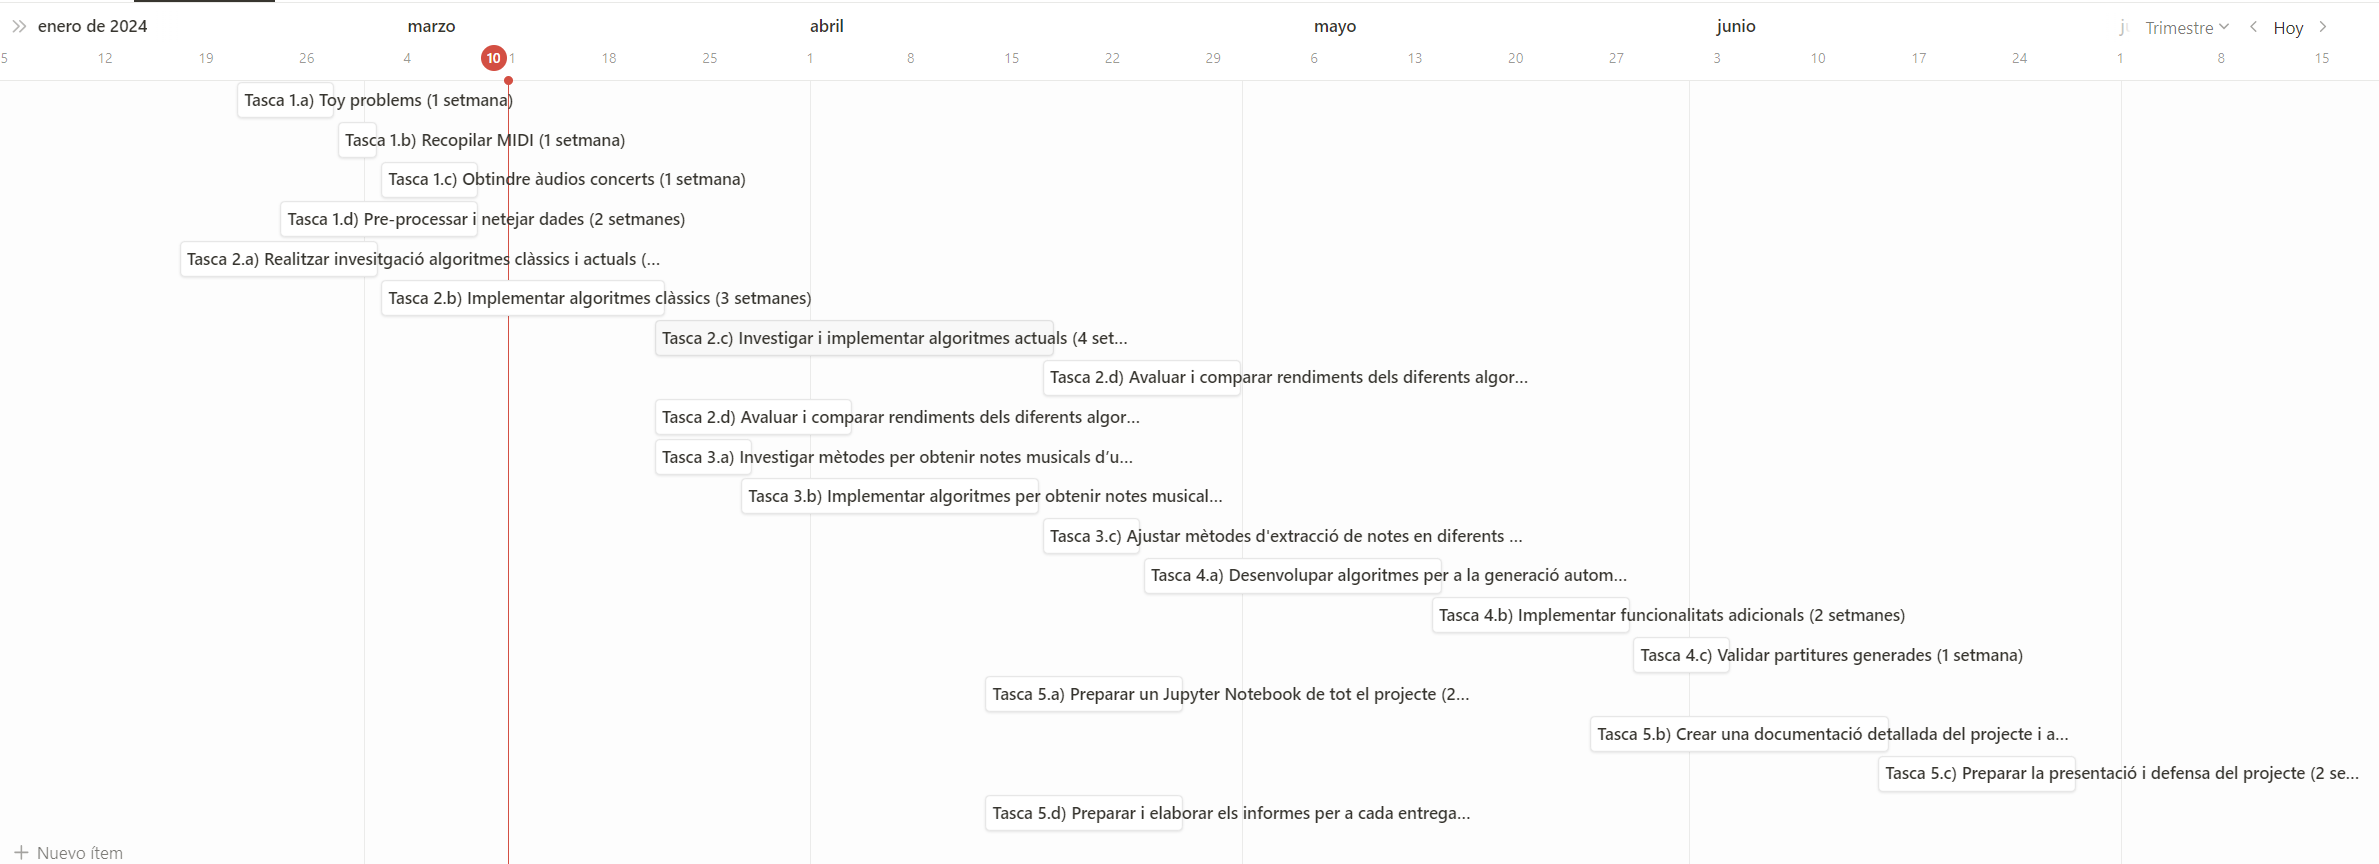
\includegraphics[width=\textwidth]{img/Diagrama de Gantt Claro Fecha.png}
    \caption{Diagrama de Gantt del projecte.}
    \label{fig:gantt}
\end{figure*}

Com es pot observar, les tasques de l'apartat 5 (documentació) són més paral·leles, és a dir, realment s'aniran realitzant durant el desenvolupament del projecte.
En total s'ha aconseguit ajustar en el plaç de temps donat tot i que per a aconseguir-ho s'haurà de realitzar alguna hora extra, sobretot en la part inicial del projecte.

\section{Desenvolupament}

El desenvolupament del projecte s'ha separat en 4 grans apartats. Inicialment, la generació i neteja de dades, a continuació, la separació d'àudio en pistes, continuant amb l'anàlisi de la pista obtenint les notes en format MIDI per a finalment generar la partitura donat aquest arxiu.

\subsection{Dades}
Les dades es separen en diferents grups segons la finalitat d'utilització de les mateixes.

\subsubsection{Elements Simples i Toy Problems}

Els elements simples consisteixen en sons senzills d'un mateix instrument tocant una sola nota o una melodia simple. La duració màxima d'aquestes dades és de 5 segons.

Aquests elements simples s'introdueixen en un bloc de codi que anomenem "generador". Aquest generador agrupa un o més elements simples per generar els \textbf{Toy Problems}. Els Toy Problems són el resultat d'agrupar els elements simples i modificar-los mitjançant els valors de diverses variables del generador. Les variables d'ajust són: \(\alpha\), \(\beta\), volum1 i volum2, amb les quals es crea i modifica un àudio estèreo per variar el volum dels canals dret i esquerre. Aquests valors permeten generar moltes dades diferents amb pocs recursos (elements simples). Per mantenir la base de dades senzilla i de petites dimensions, els Toy Problems no s'enregistren; simplement s'enregistra la seva llavor (seed) de creació, que consta dels valors de les variables i dels elements simples utilitzats.

L'esquema de creació del Toy Problem és el següent: \ref{fig:data-generator-formula}
\begin{figure}[h]
    \centering
    
\includegraphics[width=1\linewidth]{img/data_generator_formula.png}
    \caption{Esquema de creació de Toy Problems}
    \label{fig:data-generator-formula}
\end{figure}

\subsubsection{Elements Complexos i Problemes Complexos}

Els elements complexos, de manera similar als Toy Problems, es generen per formar els \textbf{problemes complexes}. Aquests problemes estan formats per melodies més complexes amb l'objectiu de tenir àudios d'entrenament més fidels a la realitat, com ara cançons del mercat o similars.

\subsubsection{Àudios Reals}

Els àudios reals consisteixen en enregistraments d'àudios com concerts, gravacions de mòbil, etc. Aquest tipus de dades només s'utilitzen per a la part de test, ja que el model no s'entrena amb aquestes dades.

En resum, el projecte utilitza 5 tipus de dades, dels quals 3 s'utilitzen per entrenar, validar i testar el model, i 1 només per a la part de test. Els 2 tipus de dades restants són elements utilitzats per generar les dades d'entrenament, validació i test.



\subsection{Separació d'àudio}

Per a la separació d'àudio, s'aplicaran dos mètodes diferents amb l'objectiu d'analitzar i comparar els resultats obtinguts.

El primer mètode utilitzat serà el mètode clàssic, basat en l'algoritme de Independent Component Analysis (ICA). L'ICA és un mètode amplament utilitzat per a la descomposició de l'audio en les seves fonts originals. Aquest algoritme té com a objectiu la separació de les senyals d'entrada en diferents components independents. En aquest cas, s'utilitzarà l'ICA per aconseguir la separació d'un àudio en pistes individuals.

D'altra banda, s'aplicarà un segon mètode basat en tècniques de Machine Learning (ML). En aquest cas, es farà servir una arquitectura de xarxa neuronal convolucional (CNN) coneguda com a U-Net \cite{spleeter2020}. La U-Net és àmpliament utilitzada en tasques de processament d'àudio i imatge per a la segmentació i reconstrucció d'imatges. Tot i que la U-Net és l'opció principal, es considerarà l'ús d'altres arquitectures de xarxes neuronals si es considera més convenient per al projecte.

Per a poder analitzar el rendiment d'aquests mètodes amb les màximes variacions possibles, s'utilitzaran diverses formes de processament d'àudio, que es programaran com a "caixes" o funcions per a permetre el seu fàcil intercanvi per tal de poder comparar els resultats finals i analitzar en quins casos funciona millor una forma de processament o si una d'elles destaca notablement respecte les altres. 

Aquestes formes de processament inclouran \cite{audio-processing-ML}:

\begin{itemize}
\item \textbf{Spectrum:} Anàlisi de l'espectre de freqüències de l'àudio.
\item \textbf{Cepstrum:} Anàlisi del cepstre de l'àudio, utilitzat per a la representació de la informació d'una manera més robusta enfront de la reverberació i el soroll.
\item \textbf{MFCC (Mel Frequency Cepstral Coefficients):} Coeficients cepstrals de les freqüències mel, amplament utilitzats en el reconeixement de veu i altres tasques de processament d'àudio.
\item \textbf{GFCC (Gammatone Frequency Cepstral Coefficients):} Coeficients cepstrals de les freqüències gammatone, una representació més semblant al processament auditiu humà.
\end{itemize}

Aquestes formes de processament permetran una anàlisi detallada dels resultats obtinguts mitjançant diferents mètodes i tècniques, ajudant a determinar quin és l'approach més adequat per al problema de separació d'àudio en el marc d'aquest projecte.

\subsection{Algoritme clàssic - Independent Component Analysis (ICA)}

L'Anàlisi de Components Independents (ICA) és un mètode computacional que permet la separació de senyals combinats en les seves fonts originals independents. En el context de descomposició d'àudio, l'ICA s'utilitza per separar mescles d'àudio en les seves components individuals.

\subsubsection{Preprocessament Inicial}

El preprocessament inicial per a l'algoritme ICA implica la recopilació de dades d'àudio mixtes, que són mescles lineals de diverses fonts d'àudio independents. Aquestes mescles es poden obtenir a partir d'experiments o de fonts d'àudio generades artificialment. Aquest últim és el meu cas principal, doncs utilitzo el generador d'àudio aleatori donats elements simples.

\subsubsection{Model Matemàtic}

El model matemàtic de l'ICA assumeix que les dades observades $\mathbf{X}$ són una mescla lineal de fonts independents $\mathbf{S}$ a través d'una matriu de mescla $\mathbf{A}$:

\begin{equation}
\mathbf{X} = \mathbf{A} \mathbf{S}
\end{equation}

L'objectiu de l'ICA és estimar les components independents $\mathbf{S}$ i la matriu de mescla $\mathbf{A}$ a partir de les dades observades $\mathbf{X}$.

\subsubsection{Aplicació de l'Algoritme ICA}

L'aplicació de l'algoritme ICA segueix aquests passos:

\begin{itemize}
    \item \textbf{Centrat i blanqueig:} Les dades d'entrada es centren (es resten les mitjanes) i es blanquegen (transformació per obtenir components no correlacionades amb variància unitària).
    \item \textbf{Estimació de components independents:} Utilitzant un algoritme iteratiu, com FastICA, es maximitza la no-Gaussianitat de les dades transformades per obtenir les components independents $\mathbf{S}$.
    \item \textbf{Reordenació i escalat:} Les components recuperades es poden reordenar i escalar per correspondre millor amb les fonts originals.
\end{itemize}

\subsubsection{Avaluació del Rendiment}

L'avaluació del rendiment de l'algoritme ICA es pot dur a terme mitjançant diverses mètriques, com ara la correlació entre les components separades i les fonts originals, el coeficient de determinació (R²), i altres mesures de qualitat de senyal.

\subsubsection{Anàlisi de Resultats i Limitacions}

Després de l'aplicació de l'algoritme ICA, els resultats obtinguts es comparen amb les fonts originals per avaluar l'eficàcia de la separació. L'anàlisi de resultats inclou la identificació de limitacions de l'algoritme, com ara la seva sensibilitat al soroll i la dificultat per separar fonts que no siguin suficientment independents.

Aquest enfocament permet una comprensió detallada de com l'algoritme ICA pot ser aplicat en la descomposició d'àudio i proporciona una base sòlida per comparar-ne el rendiment amb altres mètodes, com les xarxes neuronals convolucionals amb arquitectura U-net que es veurà més endavant.

\subsection{Algoritme actual - Machine Learning (CNN, U-net)}

El procés de desenvolupament de l'algoritme de descomposició d'àudio es basa en l'ús d'una xarxa neuronal convolucional (CNN) amb una arquitectura U-net. L'objectiu principal és entrenar el model per separar les diferents components d'un senyal d'àudio complex, format per la combinació de sons simples.

\subsubsection{Preprocessament Inicial}

Inicialment comptem amb unes dades simples (SimpleElements), que consisteixen en sons individuals d'instruments. Aquests sons es combinen aleatòriament utilitzant un generador per crear àudios complexos, denominats Toy Problems, que serviran com a dades d'entrenament. Aquest generador s'ha modificat respecte al plantejat anteriorment per a realitzar els canvis aleatòris realitzats al Toy Problem també als elements simples. D'aquesta manera s'obtenen els valors de \textit{ground truth}. Posteriorment, es divideixen els Toy Problems en tres subconjunts: entrenament, validació i test.

\subsubsection{Entrenament del Model}

L'entrenament del model implica la configuració de diversos paràmetres com el nombre de \textit{batches} d'entrenament \textit{(train\_batches)}, la mida del batch \textit{(batch\_size)} i el nombre total d'èpoques \textit{(epochs)}. Durant cada època, es segueix el següent procediment:

\begin{itemize}
    \item Per a cada \textit{batch} d'entrenament, es generen àudios complexos i els seus corresponents resultats \textit{(ground truth)} mitjançant el generador.
    \item Aquests àudios es converteixen en espectrogrames.
    \item Els espectrogrames s'ajusten a la mida adequada i es processen en forma de \textit{batch} per entrenar el model.
\end{itemize}

Després de processar els batches d'entrenament, es procedeix de manera similar amb els batches de validació per avaluar el rendiment del model durant l'entrenament.

\subsubsection{Avaluació Final}

Un cop completades totes les èpoques d'entrenament, s'utilitza el conjunt de test per avaluar el rendiment del model de manera objectiva. Les mètriques d'avaluació calculades inclouen l'exactitud, la precisió, el recall i el F1-score, entre d'altres.

\subsubsection{Anàlisi de Resultats i Ajustament del Model}

Finalment, els resultats obtinguts es revisen per identificar els punts forts i febles del model. Aquest anàlisi permet ajustar els hiperparàmetres i refinar l'arquitectura del model per millorar-ne el rendiment.

Aquest procés iteratiu assegura que el model s'entreni de manera òptima, es validi per evitar el sobreajustament i es testi per garantir una avaluació precisa del seu rendiment global.


\subsection{Anàlisi de resultats (Temporal)}

De moment no està pensat del tot aquest apartat, per tant la informació d'aquest és temporal i susceptible a canvis.

La idea principal és obtenir els resultats del punt anterior i guardar-los de manera automatitzada guardant la seed de generació de les dades d'entrada, el processament de dades i algorisme utilitzat i alguns hiperparàmetres importants per tal de poder replicar els resultats en un futur en cas de voler estudiar més un cas.

Una vegada obtingut això, per a cada experiment (Toy problems, problemes complexes i àudios reals), es calcularan algunes mètriques (les quals estàn per decidir encara) per tal de realitzar una avaluació no supervisada.

Addicionalment també es realitzarà una avaluació supervisada per mi mateix on assignaré un valor segons el rang correctesa de la separació d'àudio.

\subsection{Transcripció d'àudio}

Donada una de les pistes obtingudes en la separació d'àudio, és a dir un sol instrument, es realitza una transcripció de les notes en format MIDI. D'aquesta manera, es coneix la durada de cada nota i la seva posició temporal. \cite{music-transcription-app132111882} 

Per al desenvolupament d'aquesta part m'he basat en Omnizard \cite{Omnizard-Wu2021}, doncs ha estat amb el que he obtingut millors resultats.


\subsection{Generació de partitura}

Per a la generació de partitures, he estat fent recerca i provant les llibreries music21 \cite{music21-conf/ismir/CuthbertA10} i partitura \cite{partitura_mec}.

En aquest context, s'ha obtingut millors resultats amb la llibreria music21, però s'explorarà amb més profunditat la llibreria partitura.

L'objectiu d'aquesta subsecció és generar la partitura de cada pista o instrument obtingut mitjançant el procés de separació d'àudio.

\section{Resultats}
Per tal d'expressar de la millor manera possible els resultats, es separaràn en diverses subseccions.

\subsection{Audio Decomposition}

En aquesta secció es descriuen les mètriques utilitzades per avaluar els resultats dels algoritmes clàssic ICA i Machine Learning basat en CNN amb arquitectura U-net, així com les expectatives de rendiment de cadascun (Doncs encara no he obtingut resultats reals amb una suficient qualitat com per realitzar anàlisis exhaustius, però m'he basat en tota la informació recollida durant la recerca). Aquest anàlisi preliminar servirà com a guia per als resultats esperats i proporcionarà una base per a futurs ajustaments i millores.

\subsection{Mètriques Quantitatives}

Per avaluar la qualitat de la descomposició d'àudio, s'utilitzaran les següents mètriques quantitatives:

\begin{itemize}
    \item \textbf{Relació Senyal-Soroll (SNR):} \cite{Johnson:2006_SNR} Aquesta mètrica mesura la qualitat de la separació de les fonts. Un SNR més alt indica una millor qualitat de separació. S'espera que la CNN amb U-net tingui un SNR més alt en comparació amb l'ICA, especialment en entorns amb soroll complex i fonts no independents.
    
    \item \textbf{Correlació Creuada:} Mesura la similitud entre les fonts separades i les fonts originals. Es preveu que la CNN amb U-net mostri una correlació creuada més alta degut a la seva capacitat per capturar relacions no lineals.
    
    \item \textbf{Coeficient de Determinació (R²):} \cite{akossou2013impact_r_squared} Aquesta mètrica mesura la proporció de la variància de les fonts originals explicada per les fonts separades. S'espera que la CNN amb U-net tingui un R² més alt, indicant una millor capacitat per explicar la variabilitat en les dades d'àudio.
    
    \item \textbf{Mean Squared Error (MSE):} \cite{5937917_MSE} Mesura la diferència quadrada mitjana entre les fonts separades i les fonts originals. Es preveu que la CNN amb U-net tingui un MSE més baix en comparació amb l'ICA, suggerint una millor precisió en la separació.
\end{itemize}

\subsection{Anàlisi Qualitativa}

A més de les mètriques quantitatives, es realitzarà una anàlisi qualitativa per avaluar altres aspectes de la qualitat de la separació de les fonts:

\begin{itemize}
    \item \textbf{Qualitat Subjectiva de l'Àudio:} Es farà una avaluació de la qualitat perceptiva de les fonts separades mitjançant proves d'escolta humana. Aplicaré un rang de notes (encara per establir. Exemple: De l'1 al 5 on 1 és molt mal rendiment i 5 molt bon rendiment), d'aquesta manera es podrà quantificar també. Es preveu que les fonts separades per la CNN amb U-net siguin percebudes com a més naturals i menys distorsionades que les obtingudes amb ICA.
    
    \item \textbf{Robustesa al Soroll:} Aquesta mètrica mesura com de bé l'algoritme pot separar fonts en presència de soroll. S'espera que la CNN amb U-net sigui més robusta en entorns sorollosos gràcies a la seva capacitat per aprendre característiques complexes de les dades.
    
    \item \textbf{Capacitat de Generalització:} Es valorarà com de bé l'algoritme funciona amb dades no vistes durant l'entrenament. Si la CNN amb U-net està ben entrenada amb una varietat de dades, s'espera que tingui una millor capacitat de generalització en comparació amb l'ICA.
\end{itemize}

Aquestes dues últimes estàn pensades per realitzar-se en un futur, doncs el generador es pot millorar per implementar soroll o un desfasament, per exemple. La qual cosa podrà aportar més qualitat al processament de dades, entrenament del model i finalment a l'anàlisi de resultats.

% Petita conclusió
En resum, tot i que l'algoritme ICA és una tècnica clàssica robusta per a la separació de fonts, la CNN amb U-net és esperada a superar l'ICA en diverses mètriques clau gràcies a la seva capacitat per aprendre característiques complexes i no lineals de les dades d'àudio. La CNN amb U-net oferirà probablement una millor qualitat de separació, robustesa al soroll i capacitat de generalització, fent-la una opció més adequada per a tasques de descomposició d'àudio en entorns complexos.


\subsection{Resultats - Altres parts (Temporals)}

Actualement, s'ha aconseguit realitzar l'esquelet de tot el procés, és a dir, donat un àudio, s'obtenen diverses pistes amb els diversos instruments. Una vegada obtinguts, si s'introdueix un àudio, mitjançant Omnizard (que permet introduir links de Youtube o arxius .mp3), s'obté la pista en format MIDI. Finalment, amb la llibreria Music21, s'obté la partitura.

A continuació mostraré links de diversos Google Colab amb exemples d'aquestes proves i resultats, així com algunes imatges.

\subsection{Audio Decomposition Part}

Google Colab: \href{https://colab.research.google.com/drive/1hnlwqaULE_wZDV8ZtSGldOrITDW8WQJs?usp=sharing}{Google Colab Audio Decomposition Part}
En aquesta part, s'introdueix un àudio, que per a l'exemple és de 10 segons, i mitjançant Spleeter \cite{spleeter2020}, es separa en les diverses pistes.

També es pot veure que vaig intentar realitzar una integració amb Omnizard però va fallar per alguna incompatibilitat. És per això que ho vaig separar amb la següent part.

\subsection{Transcripció musical i generació de partitura}

Google Colab 1: \href{https://colab.research.google.com/drive/1W1kDEtN0w8kRLiUZLePwhXBxqFlJAA4x?usp=sharing}{Transcripció (Generació de fitxer MIDI)}
Google Colab 2: \href{https://colab.research.google.com/drive/1tiGLzMGYfOxaYQx5lRwElC0yLjdWvwAU?usp=sharing}{Generació de Partitura}

Per a seguir amb la segona i última part, mitjançant el Google Colab 1, generem l'arxiu en format MIDI donat un arxiu MP3 o un link de Youtube.
La prova la vaig realitzar amb aquest link: \href{https://www.youtube.com/watch?v=aCUI6dNECeA&ab_channel=tocapartituras.com}{Link cançó piano YT}

Com es pot observar, s'obté un fitxer MIDI de manera correcta. El que vaig fer a continuació va ser obrir i escoltar aquest arxiu i tret d'algunes diferències, en general el resultat era bastant fidedigne amb l'original.

A continuació, mitjançant el Google Colab 2, introduim el fitxer prèviament generat (MIDI) per a obtenir la respectiva partitura.
Imatge de la partitura original: \ref{fig:paritura-original}
\begin{figure}[h]
    \centering
    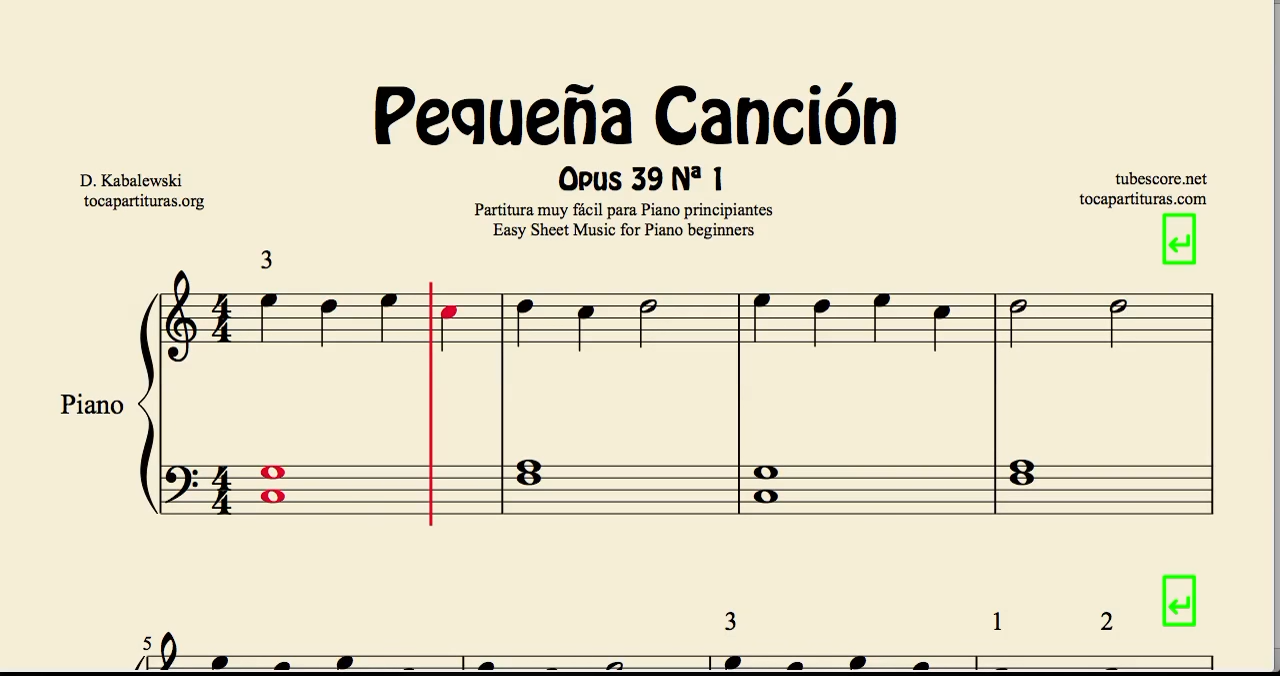
\includegraphics[width=1\linewidth]{img/screenshot-partitura-correcta.png}
    \caption{Partitura original del video de YouTube}
    \label{fig:paritura-original}
\end{figure}

I a continuació podem veure la partitura generada: \ref{fig:partitura-resultat}
\begin{figure}[h]
    \centering
    
\includegraphics[width=1\linewidth]{img/partitura_resultat.png}
    \caption{Partitura resultant, generada al Google Colab 2.}
    \label{fig:partitura-resultat}
\end{figure}

Com es pot observar, el resultat és desastrós i molt diferent. Tot i això es veu que és possible una generació de partitura, tot i que se li haurà de dedicar més temps a entendre com funciona. Ja que, per exemple, es pot veure que la partitura inicial compta amb melodia en la mà dreta i la mà esquerra. En canvi, en la partitura resultant, només ha considerat la de la mà dreta. Aquest podria ser el punt principal d'error fent que es desquadri tant.

Utilitzant la mateixa llibreria i en un entorn controlat, es pot obtenir un resultat correcte, tal i com es pot veure a continuació: \ref{fig:partiture-example}
\begin{figure}[h]
    \centering
    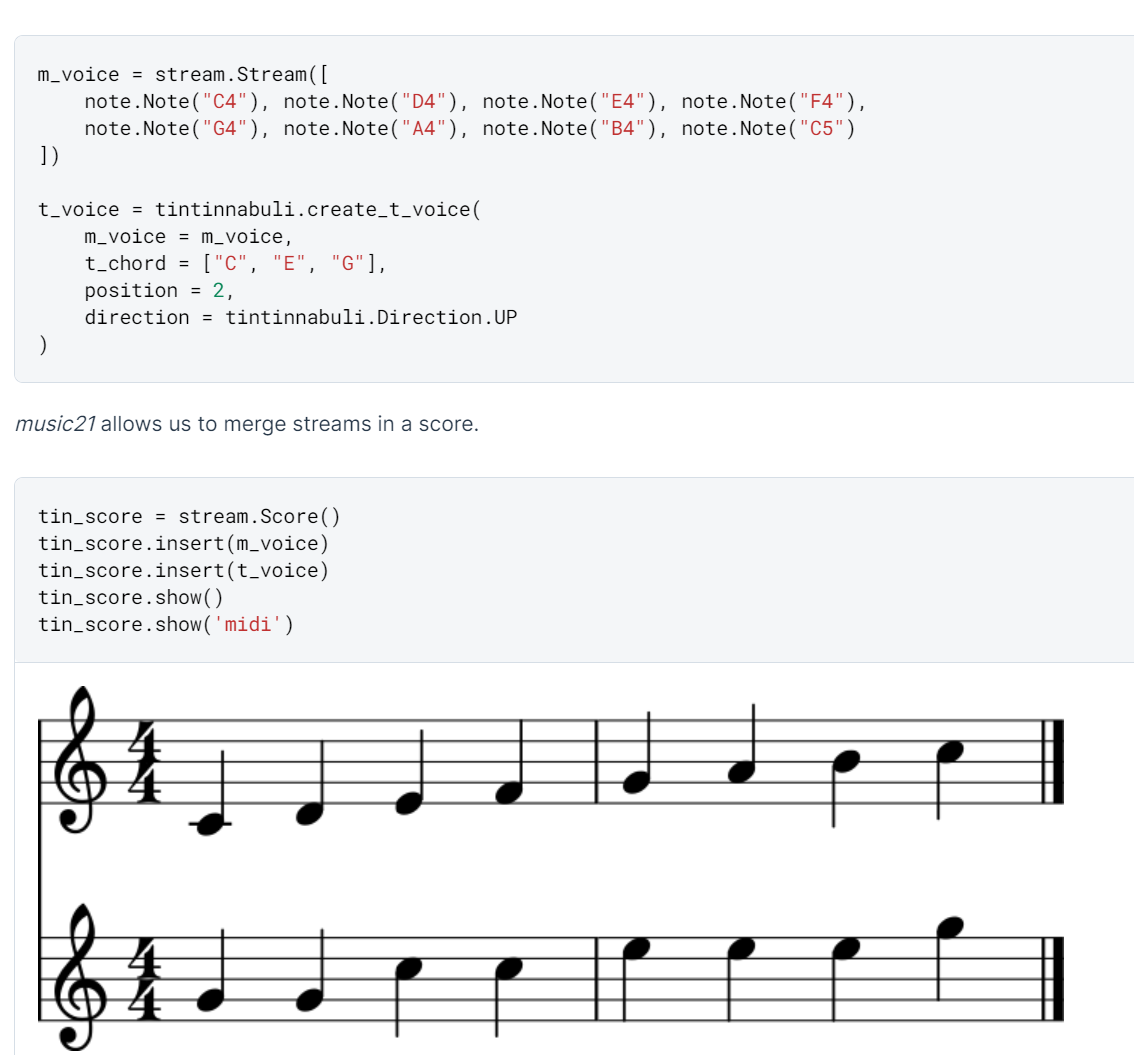
\includegraphics[width=1\linewidth]{img/Partiture-Example.png}
    \caption{Exemple de generació de Partitura en un entorn controlat}
    \label{fig:partiture-example}
\end{figure}


\subsection{Resultats reals - ICA}

Per a l'execució de l'algorisme d'ICA, es generen Toy Problems mitjançant elements simples. Cal destacar que un Toy Problem consta de 2 elements simples. Posteriorment, l'àudio es converteix en espectrogrames per facilitar l'aplicació de l'algorisme ICA i l'obtenció dels resultats.

Els resultats inclouen dos conjunts d'arxius, dos arxius de ground truth generats pel generador de Toy Problems i dos arxius més creats pel propi algoritme (resultat d'execució).

L'anàlisi i revisió supervisada de l'àudio confirma que l'algorisme clàssic no és completament eficient en la separació d'àudio. La versió desenvolupada, tot i semblar-se al Ground Truth, presenta soroll considerable que dificulta la distinció clara dels instruments. Això suggereix que la separació pot no estar realitzant-se de manera adequada.

A més de l'anàlisi supervisada, s'ha realitzat una comparació visual dels espectrogrames resultants de l'execució de l'ICA amb els Ground Truth.

\begin{figure}[h]
    \centering
    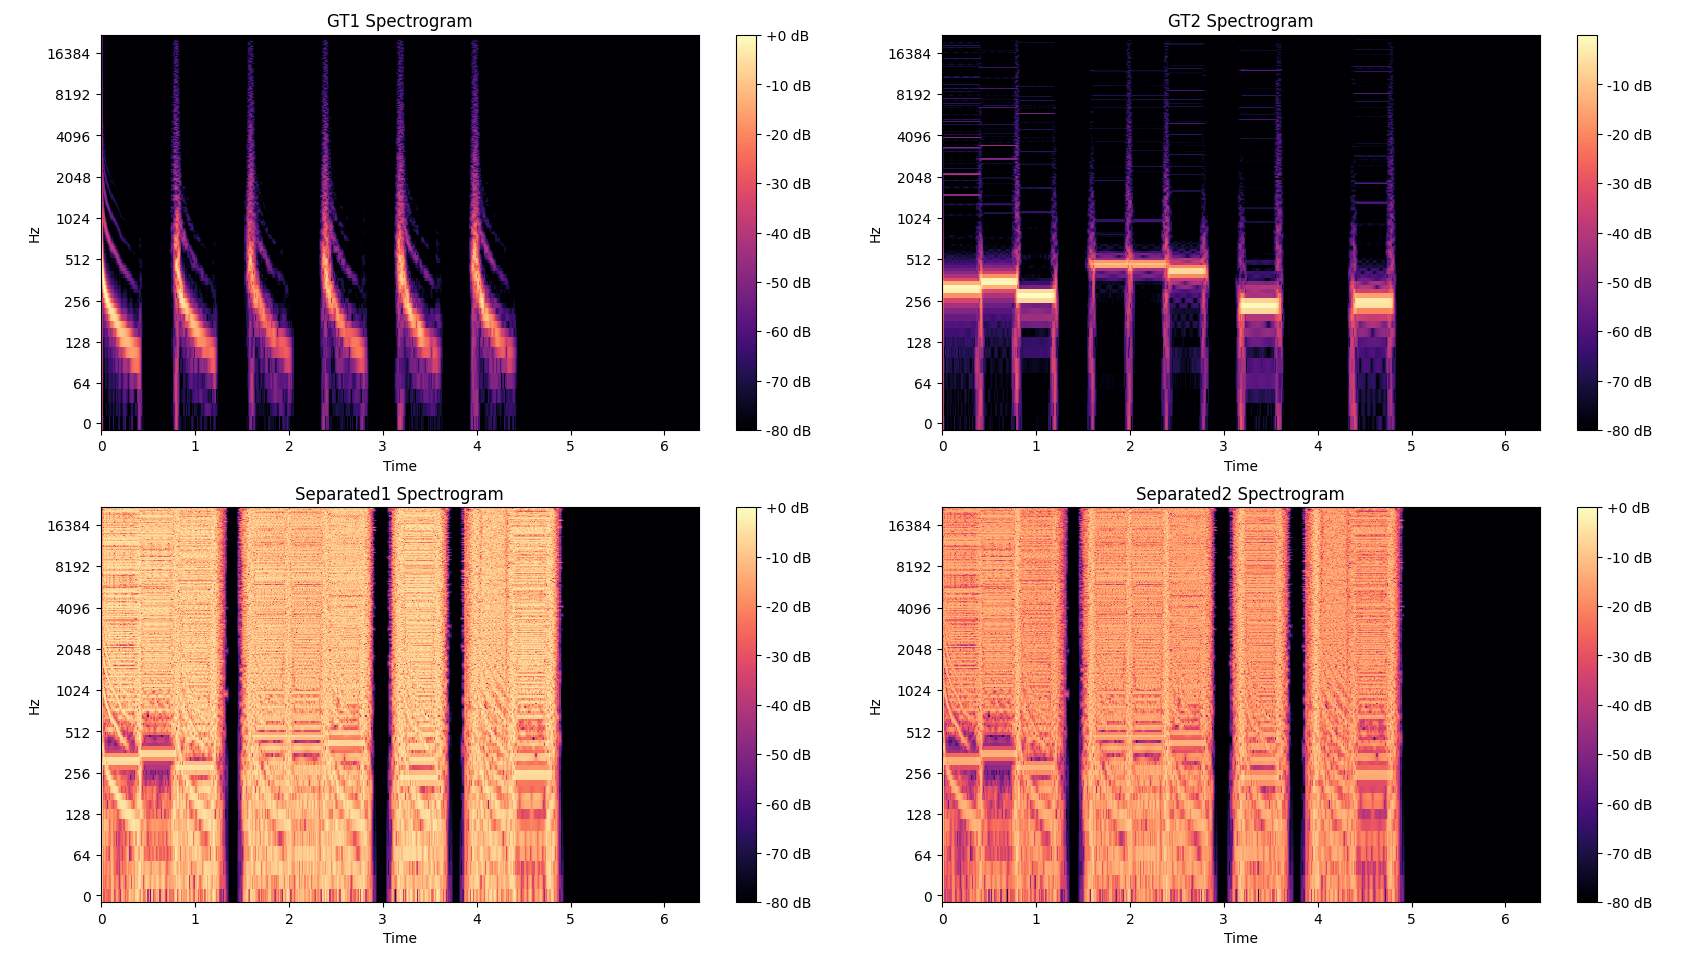
\includegraphics[width=1\linewidth]{img/ica_results/ica_results_spectogram_example_1.png}
    \caption{Exemple 1 d'un resultat de l'execució de l'algorisme ICA (Visualització i comparació d'espectrogrames).}
    \label{fig:ica_results-example1}
\end{figure}

Tal i com podem observar visualment, els dos espectrogrames corresponents al resultat són pràcticament iguals entre si, tret de petites variacions o d'un cert soroll.
Entenent el funcionament esperat, que era la separació de les pistes d'àudio, s'observa que no s'ha complert aquest fet, doncs més aviat semblen l'agrupació dels dos Ground Truth.

A continuació mostraré dos exemples més on el Ground Truth 2 generat és molt semblant per als dos exemples, doncs s'ha utilitzat el mateix element simple aplicant certes variacions per a la generació dels Toy Problems. El primer element simple és diferent per tal que s'observi la diferència.

\begin{figure}[h]
    \centering
    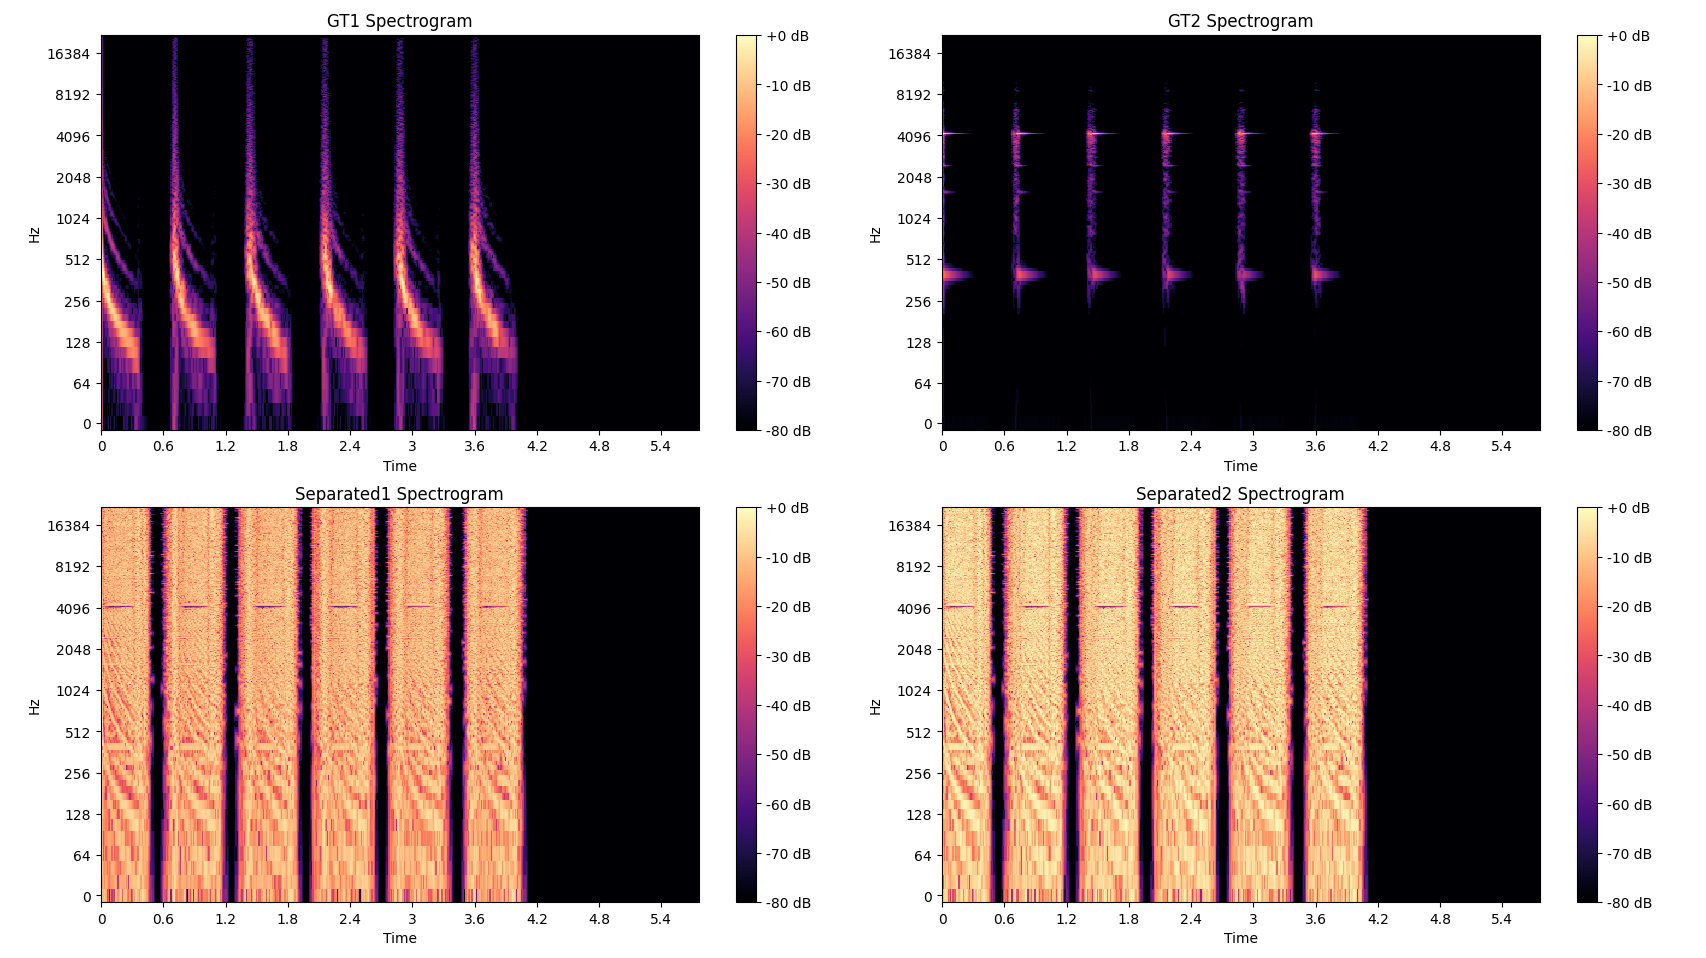
\includegraphics[width=1\linewidth]{img/ica_results/ica_results_spectogram_example_2.png}
    \caption{Exemple 2 d'un resultat de l'execució de l'algorisme ICA (Visualització i comparació d'espectrogrames).}
    \label{fig:ica_results-example2}
\end{figure}


\begin{figure}[h]
    \centering
    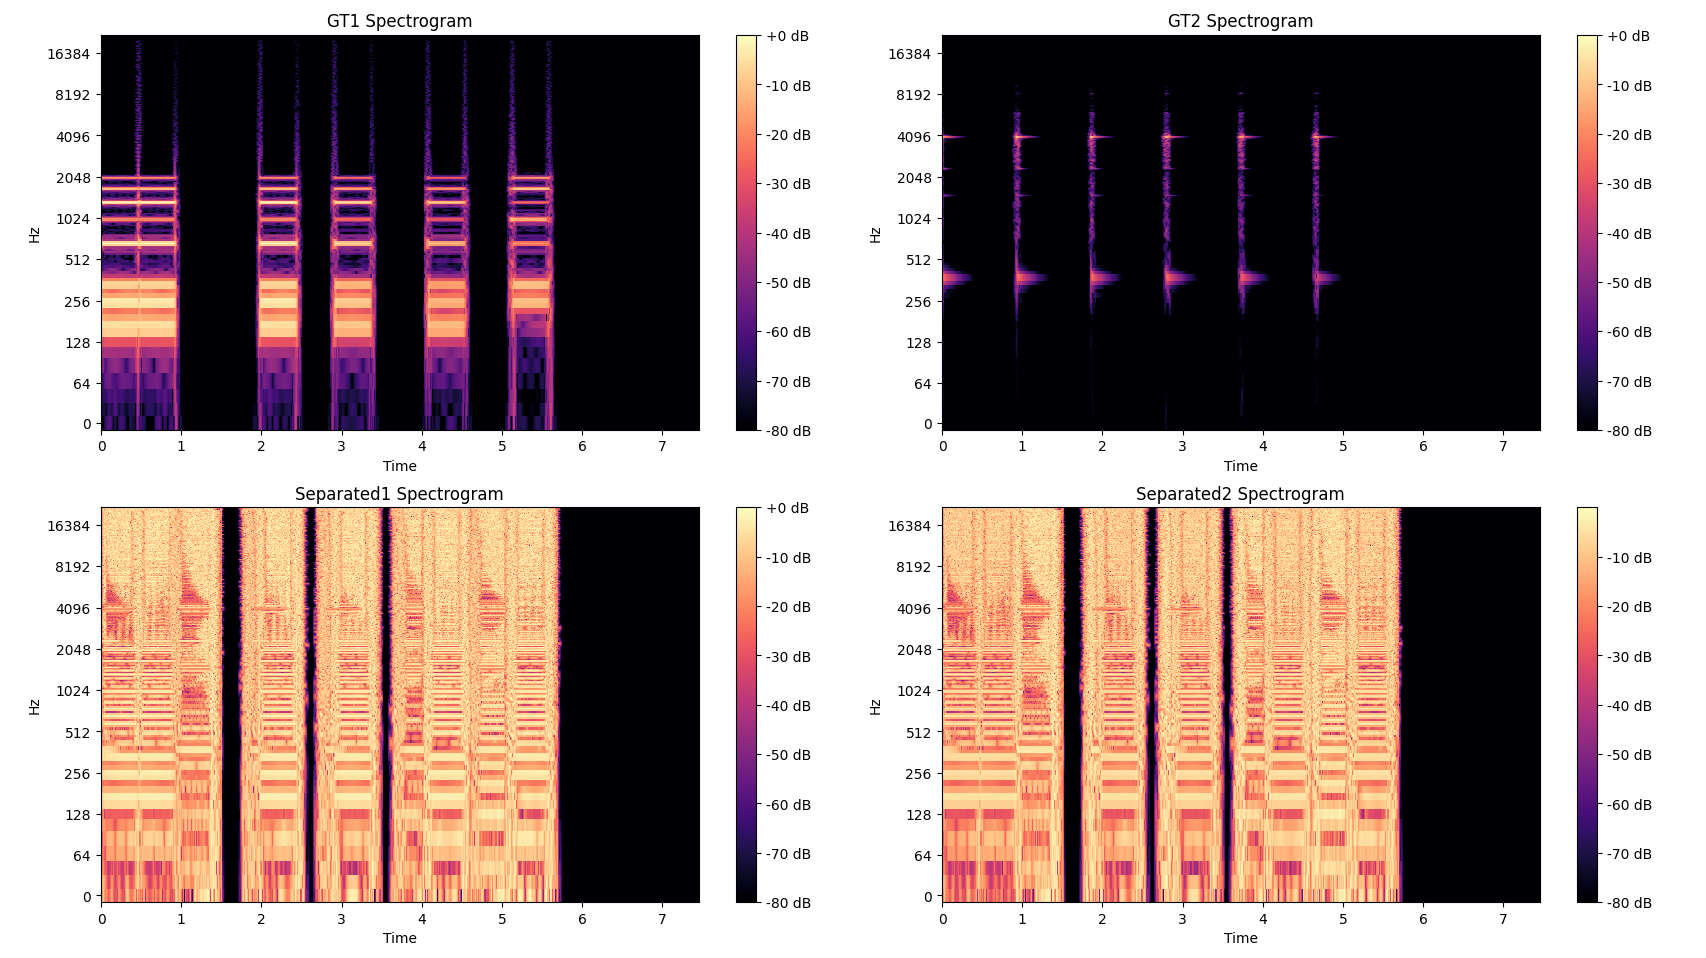
\includegraphics[width=1\linewidth]{img/ica_results/ica_results_spectogram_example_3.png}
    \caption{Exemple 3 d'un resultat de l'execució de l'algorisme ICA (Visualització i comparació d'espectrogrames).}
    \label{fig:ica_results-example3}
\end{figure}

Tal i com es pot confirmar amb aquesta nova informació, el resultat de l'ICA no és el que coneixem com separació d'àudio en pistes i, per tant, no és de suficient qualitat com per a acomplir l'objectiu esperat.

\section{Conclusions}

Tot i que encara no s'han obtingut tots els resultats, les conclusions d'aquest projecte són les següents:

L'algorisme ICA és un mètode clàssic que va ser pioner i efectiu en la seva època inicial d'implementació. Tot i que proporciona una certa distinció i separació de les pistes, la seva qualitat no és excel·lent. Per aquell temps, era suficient per discernir les diferències, tot i que el soroll podia ser evident; un arxiu resultant encara podia identificar principalment un únic instrument en l'àudio.

No obstant això, com s'ha esmentat, la seva qualitat general és limitada. Això ha portat al desenvolupament i la adopció de noves tecnologies, com els models basats en aprenentatge automàtic, que ofereixen una millor qualitat i precisió.

En aquest projecte, s'ha optat per utilitzar un model actual basat en l'arquitectura U-Net, el qual ha demostrat ser eficaç per a la segmentació d'imatges. Encara que aquest model està dissenyat per a imatges, s'ha aplicat a àudio transformant-lo prèviament en format d'espectrograma.

Aquesta decisió ha comportat diversos reptes i complicacions. La transformació d'àudio a un format d'imatge adient per a la entrada del model U-Net no és trivial, especialment per a algú sense experiència prèvia.

Així doncs, és essencial considerar els reptes potencials abans d'emprendre un projecte d'aquest tipus. Per a un principiant com jo, la implementació d'aquest model ha representat un desafiament considerable.

Per tant, és important reconèixer que l'algorisme ICA, malgrat les seves limitacions, és més senzill d'implementar, tot i que els resultats poden ser inferiors. En contrapartida, models més avançats com l'arquitectura U-Net prometen resultats superiors, però la seva implementació pot ser notablement més complexa.

No sempre uns resultats superiors es tradueixen en una major complexitat d'implementació; sovint reflecteixen tècniques més eficaces i millor desenvolupades. Tanmateix, en el meu cas personal, la implementació d'aquest model ha implicat una dificultat addicional significativa.


\section*{Agraïments}

... ..  .... .. .... ... ..... ... ..... ... ... ..... .... .
.... ..  .... .. .... ... ..... ... ..... ... ... ..... .... .
.... ..  .... .. .... ... ..... ... ..... ... ... ..... .... .
.... ..  .... .. .... ... ..... ... ..... ... ... ..... .... .
.... ..  .... .. .... ... ..... ... ..... ... ... ..... .... .


\bibliographystyle{plain}
\bibliography{biblio}


\appendix

\section*{Apèndix}

\setcounter{section}{1}

\subsection{Secció d'Apèndix}


... ..  .... .. .... ... ..... ... ..... ... ... ..... .... .
.... ..  .... .. .... ... ..... ... ..... ... ... ..... .... .
.... ..  .... .. .... ... ..... ... ..... ... ... ..... .... .
.... ..  .... .. .... ... ..... ... ..... ... ... ..... .... .
.... ..  .... .. .... ... ..... ... ..... ... ... ..... .... .

\subsection{Secció d'Apèndix}


... ..  .... .. .... ... ..... ... ..... ... ... ..... .... .
.... ..  .... .. .... ... ..... ... ..... ... ... ..... .... .
.... ..  .... .. .... ... ..... ... ..... ... ... ..... .... .
.... ..  .... .. .... ... ..... ... ..... ... ... ..... .... .
.... ..  .... .. .... ... ..... ... ..... ... ... ..... .... .


\end{document}

